%%% PREAMBLE - Do not touch %%%%%%%%%%%%%%%%%%%%%%%%%%%%%%%%%%%%%%%%%%%%%%%%%%%%%%
\documentclass[10pt,twocolumn,letterpaper]{article}
%%\usepackage[ansinew]{inputenc}
\usepackage[latin1,utf8]{inputenc}
\usepackage[portuges,brazil,english]{babel}
\usepackage{model}
\usepackage{times}
\usepackage{epsfig}
\usepackage{graphicx}
\usepackage{amsmath}
\usepackage{amssymb}
\usepackage{color}
\usepackage[pagebackref=true,breaklinks=true,letterpaper=true,colorlinks,bookmarks=false]{hyperref}
%  ABACO -- Conjunto de macros para desenhar o 'abaco

%  Desenho original de Hans Liesenberg

%  Macros de Tomasz Kowaltowski

%  DCC -- IMECC -- UNICAMP

%  Mar,co de 1988  --  Vers~ao 1.0

% Ajustado para LaTeX da SUN -- Mar,co de 1991

% ---------------------------------------------------------

%  Chamada:   \ABACO{d1}{d2}{d3}{d4}{esc}
%             com:  di's -- os quatro d'igitos;
%	           esc  -- fator de escala

% ---------------------------------------------------------

%  DEFINI,C~OES AUXILIARES

% ---------------------------------------------------------


%  Forma o d'igito pequeno (0 ou 1)

\newcommand{\ABACODP}[1]{%
%
\thicklines
%    
\begin{picture}(8,0)
    \ifcase#1{   %  caso 0
       \put(0,0)    {\line(1,0){4}}
       \multiput(5,0)(2,0){2}{\oval(2,4)}}
    \or{         %  caso 1
       \put(2,0)    {\line(1,0){4}}
       \multiput(1,0)(6,0){2}{\oval(2,4)}}
    \fi
\end{picture}
    } % \ABACODP

% Forma o d'igito grande (0 a 4)

\newcommand{\ABACODG}[1]{%
%
\thicklines
%    
\begin{picture}(14,0)
    \ifcase#1{   % caso 0
       \multiput(1,0)(2,0){5}{\oval(2,4)}}
       \put(10,0)   {\line(1,0){4}}
    \or{         % caso 1
       \multiput(1,0)(2,0){4}{\oval(2,4)}}
       \put(8,0)   {\line(1,0){4}}
       \put(13,0)   {\oval(2,4)}
    \or{         % caso 2
       \multiput(1,0)(2,0){3}{\oval(2,4)}
       \put(6,0)   {\line(1,0){4}}
       \multiput(11,0)(2,0){2}{\oval(2,4)}}
    \or{         % caso 3
       \multiput(1,0)(2,0){2}{\oval(2,4)}
       \put(4,0)   {\line(1,0){4}}
       \multiput(9,0)(2,0){3}{\oval(2,4)}}
    \or{         % caso 4
       \put(1,0)  {\oval(2,4)}}
       \put(2,0)   {\line(1,0){4}}
       \multiput(7,0)(2,0){4}{\oval(2,4)}
    \fi
\end{picture}
    } % \ABACODG
       
% Forma um d'igito (0 a 9)

\newcommand{\ABACOD}[1]{%
%
    \ifnum#1>9
       \errmessage{#1: Argumento invalido para ABACO}
    \fi
    \ifnum#1<0
       \errmessage{#1: Argumento invalido para ABACO}
    \fi
%
\begin{picture}(24,0)
%    
    \ifnum#1<5
       \put(16,0) {\ABACODP{0}}
    \else   
       \put(16,0) {\ABACODP{1}}
    \fi
%    
    \ifnum#1<5
       \put(0,0)  {\ABACODG{#1}}
    \else
       \ifcase#1\or \or \or \or
          \or  \put(0,0)  {\ABACODG{0}}
          \or  \put(0,0)  {\ABACODG{1}}
          \or  \put(0,0)  {\ABACODG{2}}
          \or  \put(0,0)  {\ABACODG{3}}
          \or  \put(0,0)  {\ABACODG{4}}
       \fi
    \fi   
\end{picture}
    } % \ABACOD
    
% -------------------------------------------------

%  DEFINI,C~AO PRINCIPAL
    
\newcommand{\ABACO}[5]{%
    \setlength{\unitlength}{#5mm}
%
    \thinlines
%   
\begin{picture}(28,25)
%   
% moldura
%
% externa
%
        \put(0,0)            {\line(0,1){25}}
        \put(0,0)            {\line(1,0){28}}
        \put(28,0)           {\line(0,1){25}}
        \put(0,25)           {\line(1,0){28}}
% interna
        \put(2,2)            {\line(0,1){21}}
	\put(26,2)           {\line(0,1){21}}
	\put(16,2)           {\line(0,1){21}}
	\put(18,2)           {\line(0,1){21}}
	\put(2,2)            {\line(1,0){14}}
	\put(16,2)           {\line(1,-1){1}}
	\put(17,1)           {\line(1,1){1}}
	\put(18,2)           {\line(1,0){8}}
	\put(2,23)           {\line(1,0){14}}
	\put(16,23)          {\line(1,1){1}}
	\put(17,24)          {\line(1,-1){1}}
	\put(18,23)          {\line(1,0){8}}
	\put(0,0)            {\line(1,1){2}}
	\put(0,25)           {\line(1,-1){2}}
	\put(28,0)           {\line(-1,1){2}}
	\put(28,25)          {\line(-1,-1){2}}
%
%   
% d'igitos
%
%   
       \put(2,20)  {\ABACOD{#1}}
       \put(2,15)  {\ABACOD{#2}}
       \put(2,10)  {\ABACOD{#3}}
       \put(2,5)   {\ABACOD{#4}}
%      
\end{picture}
    } % \ABACO
    


\cvprfinalcopy % *** Uncomment this line for the final submission
\def\httilde{\mbox{\tt\raisebox{-.5ex}{\symbol{126}}}}
\ifcvprfinal\pagestyle{empty}\fi

\newcommand{\TODO}[1]{TODO: #1}
\newcommand{\CITEONE}[2]{\mbox{#1 \cite{#2}}}
\newcommand{\CITETWO}[3]{\mbox{#1 and #2 \cite{#3}}}
\newcommand{\CITEN}[2]{\mbox{#1 et al. \cite{#2}}}

%%% Paper beginning %%%%%%%%%%%%%%%%%%%%%%%%%%%%%%%%%%%%%%%%%%%%%%%%%%%%%%%%%%%%%%
\begin{document}

%%% Title and authors %%%%%%%%%%%%%%%%%%%%%%%%%%%%%%%%%%%%%%%%%%%%%%%%%%%%%%%%%%%%
\title{Printer ballistics through character's texture analysis}
\author{Adriano Ruggero\thanks{Institute of Computing, University of Campinas (Unicamp). \textbf{Contact}: \tt\small{arruggero@lasca.ic.unicamp.br}}\\
Gabriel Rodrigues\thanks{Institute of Computing, University of Campinas (Unicamp). \textbf{Contact}: \tt\small{gabriel\_rodrigues@aol.com}}\\
Mário Brito\thanks{Institute of Computing, University of Campinas (Unicamp). \textbf{Contact}:
\tt\small{britomar@aedu.com}}\\
Maurício Perez\thanks{Institute of Computing, University of Campinas (Unicamp). \textbf{Contact}:
\tt\small{mauriciolp84@gmail.com}}\\
Anderson Rocha\thanks{Institute of Computing, University of Campinas (Unicamp). \textbf{Contact}: \tt\small{anderson.rocha@ic.unicamp.br}}
}

%%% Abstract %%%%%%%%%%%%%%%%%%%%%%%%%%%%%%%%%%%%%%%%%%%%%%%%%%%%%%%%%%%%%%%%%%%%%
\maketitle
\begin{abstract}
We describe a technique for ballistics of printed documents, that is, link a printed document to a specific printer. The principle of this technique is the analysis of character's texture, by extracting some properties from the characters of the scanned images from the printed documents, and relate this properties through a co-occurrence matrix. This matrix can be used to create a "fingerprint" for the characters related to the same printer, what allows us to identify the specific printer device that printed these characters.
\end{abstract}

%%% Introduction %%%%%%%%%%%%%%%%%%%%%%%%%%%%%%%%%%%%%%%%%%%%%%%%%%%%%%%%%%%%%%%%%
\section{Introduction}
In August of 2013, a russian man wrote his own small print in a credit card contract~\cite{RT}. The credit card's administrator bank didn't read the amendments made by the client, and just signed and certified the document. The changes included unlimited credit line, 0 percent interest rates and no fees. When the bank decided to terminate the man's credit card, because overdue payments, he sued them for more than 24 million rubles (US\$ 727.000). How could the bank prove the falsification?

Altough we are living in a digital era, printed documents still are a significant part of our day by day. Likewise, with the constant reduction in prices and increase in quality of printing equipment, forgeries become increasingly commonplace.

Legal aspects aside, a way to verify if a document, or a part of it, came from a specific device can be through  character's texture analysis.

Our approach for the analysis of character's texture is as follows. From printed pages scanned at high resolution, selected characters were extracted. From these characters, we obtained its properties of contrast, correlation, energy and homogeneity, creating with them a co-occurrence matrix. This matrix can be called a ''fingerprint'' of the character. This ''fingerprint'' of  characters is closely related to the printing device which originated it, and can be used to identify which printer was responsible for printing it.

However, slight imperfections may occur during the printing and/or scanning process of documents. To handle these small errors (or variations), characters were selected from different areas of scanned document, their properties were obtained and then classified using machine learning algorithms.


%%% Add section %%%%%%%%%%%%%%%%%%%%%%%%%%%%%%%%%%%%%%%%%%%%%%%%%%%%%%%%%%%%%%%%%%
\section{State-of-the-Art}
Related work: \cite{Bulan}

%%% Add section %%%%%%%%%%%%%%%%%%%%%%%%%%%%%%%%%%%%%%%%%%%%%%%%%%%%%%%%%%%%%%%%%%
\section{Proposed Solution}

Our solution consist in getting the image of characters selected from scanned documents in grayscale, extract its properties of contrast, correlation, energy and homogeneity - creating a co-occurrence matrix - and cluster them by machine learning algorithms.

\subsection{Printers dataset}

The documents used for this work were obtained from the Wikipedia site~\cite{Wikipedia}, and were written in English, some of them containing pictures, some not. They were printed by printers listed in Table \ref{tab:printers}. 

\begin{table}
\label{tab:printers}
\caption{Printers used in this work}
\begin{center}
\begin{tabular}{l*{2}{c}r}
Printer           & Documents \\
\hline
Brother-HL4070CDW & 28 \\
Canon-D1150 & 28 \\
Canon-MF3240 & 28 \\
Canon-MF4370DN & 28 \\
HP-CLJ-CP2025A & 28 \\
HP-CLJ-CP2025B & 28 \\
HP-JL-CP1518 & 28 \\
Lexmark-E260D & 28 \\
OKI-C330 & 28 \\
Samsung-CLP315 & 28 \\
\end{tabular}
\end{center}
\end{table}

These documents were scanned at high resolution and saved as Tiff file format (Tagged Image File Format), forming a database. These files were made available through an FTP site~\cite{Printers_dataset}. An example of a typical document used in this study can be seen in Figure \ref{fig:document}.

\begin{figure}
\begin{center}
	\includegraphics[width=0.99\columnwidth]{document}
	\caption{Typical document used in this work~\cite{Wikipedia}.}
\label{fig:document}   
\end{center} 
\end{figure}

\subsection{Characters}

The characters chosen for this work were "e" and "t", both in lowercase, because they are, respectively, the first and second most common letters in texts written in English~\cite{Letter_Frequency}.

\subsection{Printers}

Due to the fact that all scanned documents come from laser printers, it was necessary to take some precautionary measures. Laser printers are known as ''page printers'', while dot matrix printers and inkjet printers are called ''line printers''. This is a crucial difference, and should be considered for more careful study. Line printers print documents line by line from the top of the sheet, keeping a characteristic pattern which periodically repeats for each paper feed. That is, any line printed by this printer model will have basically the same characteristics, regardless of their vertical location in the sheet of paper. Page printers, instead, do not print documents line by line. In this case, an image of the entire page is ''printed'' on the photoreceptor drum by a laser unit. This image attracts toner particles, and then transfers it to the paper sheet. Finally a fuser unit heats the paper, so the toner melts and attach it. Figure \ref{fig:page_printer} shows a default page printer schema.

\begin{figure}
\begin{center}
	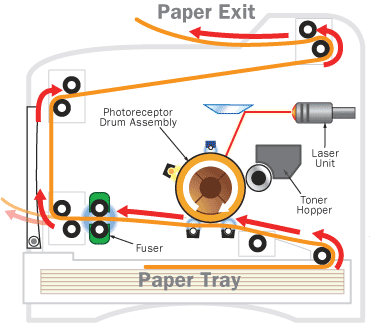
\includegraphics[width=0.99\columnwidth]{page_printer}
	\caption{Default page printer schema~\cite{Document_Analysis}.}
\label{fig:page_printer}   
\end{center} 
\end{figure}

By working in this way, page printers do not maintain a characteristic pattern that is repeated line by line across the printed sheet of paper. Due to small imperfections that may exist in the photoreceptor drum, each print area generated by this type of device can present different characteristics.
Taking into account this fact, it was necessary to obtain characters from different parts of the scanned document. Basically, each document has roughly divided into three parts: upper, middle, and bottom. The Figure \ref{fig:document_areas} shows an example of a document divided in this way. If this article is being viewed in color, the upper part of the figure is in red, the middle, in green and bottom, in blue.

\begin{figure}
\begin{center}
	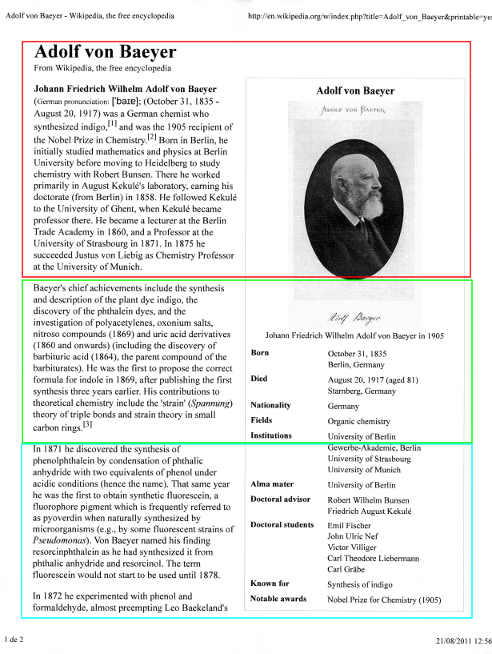
\includegraphics[width=0.99\columnwidth]{document_areas}
	\caption{Division of the scanned document in areas.}
\label{fig:document_areas}   
\end{center} 
\end{figure}

Despite showing subtle differences between characters located in different areas of the printout, the print device maintains certain intrinsic characteristics unchanged in all printed characters. Such characteristics can be compared to our fingerprints, making it a way to link a printed character to a particular device.

%%% Add section %%%%%%%%%%%%%%%%%%%%%%%%%%%%%%%%%%%%%%%%%%%%%%%%%%%%%%%%%%%%%%%%%%
\section{Experiments and Discussion}

%%% Add section %%%%%%%%%%%%%%%%%%%%%%%%%%%%%%%%%%%%%%%%%%%%%%%%%%%%%%%%%%%%%%%%%%
\section{Conclusions and Future Work}


%%% References %%%%%%%%%%%%%%%%%%%%%%%%%%%%%%%%%%%%%%%%%%%%%%%%%%%%%%%%%%%%%%%%%%%
{\small
\bibliographystyle{unsrt}
\bibliography{references_printer}
}

\end{document}
